\section{Background and Context}
\label{sec:background}


%% We represent the
%% intermediate representation in the form of a Clocked Control
%% Data Flow Graph and use LLVM language. Both these choices do
%% not add any unnecessary complexity to our formal
%% reasoning. We now provide an overview of our intermediate
%% representation and the loop pipelining transformation done
%% in behavioral synthesis tools.

\subsection{Intermediate Representation}
\label{subsec:ir}

%We represent the intermediate design in the form of a Clocked Control Data Flow Graph (CCDFG)~\cite{rhcxy:atva-09}. 
A behavioral synthesis tool performs a number of compiler
and scheduling transformations (including pipelining, which is the focus of this paper). Certification of behavioral
synthesis transformations thus requires a formalization of
the design representation manipulated by these
transformations. The formalization we use is {\em Clocked
  Control Data Flow Graph} (CCDFG)~\cite{rhcxy:atva-09}. It
is a natural formalization of an intermediate design
representation used by most behavioral synthesis tools.
Structurally, a CCDFG is a control and data flow graph augmented with a schedule.
% We use a structure called CCDFG to formalize internal
% respresentations of designs generated by behavioral
% synthesis tools(CCDFG)~\cite{rhcxy:atva-09}. Thus, our
% algroithm accepts CCDFG for sequential design and
% generates a pipelined CCDFG. A CCDFG is a Control Data
% Flow Graph augmented with a schedule.
The control flow is broken into basic blocks. The instructions are grouped into microsteps which can be executed concurrently. A scheduling step represents a group of microsteps which can be executed in a single clock cycle. State of a CCDFG at a particular microstep is a list of all the variables of a CCDFG with their corresponding values. 
%% CCDFG is a
%% natural formalization of internal representation structure
%% used in behavioral synthesis tools.

The semantics of CCDFG require a formalization of the
underlying language used to represent the individual
instructions in a scheduling step.  The underlying language we use
is the LLVM language~\cite{llvm}. LLVM is a popular compiler
infrastructure for many behavioral synthesis tools
({\em e.g.}, AutoESL~\cite{autoesl}, xPilot~\cite{xpilot},
LegUp~\cite{legup}).  We provide semantics to these
instructions through a standard, state-based operational
formalization~\cite{McCarthy}. It includes assignment,
load, store, bounded arithmetic, bit vectors, arrays, and
pointer manipulation instructions. Executing a microstep in
a CCDFG implies changing the current state of CCDFG based on
meaning of the instructions in the microstep and producing a
new state. Assigning meanings to most instructions is
standard; one exception is the so-called ``$\phi$-construct''. A $\phi$-construct is a list of $\phi$-statements. A $\phi$-statement is $v := \phi [\sigma, X] [\tau, Y]$, where $v$ is a variable, $\sigma$
and $\tau$ are expressions, and $X$ and $Y$ are
scheduling steps: if it is reached from $X$ then it is the
same as the assignment statement $v := \sigma$; if
reached from $Y$, it is the same as $v := \tau$; the meaning is undefined otherwise. $\phi$-constructs are necessary due to the structure of the SSA (static single
assignment) form of the LLVM code.

\subsection{Loop Pipelining Transformation}
\label{subsec:loop-pipelining-trans}
A behavioral synthesis tool automatically generates a RTL design from an ESL design through a series of
transformations. Pipelining a loop is a critical
transformation in behavioral synthesis. For our purposes, a
{\em pipelinable loop} is a loop with the following additional restrictions~\cite{hrx:dac-12}:
\begin{enumerate}
\item no nested loop;
\item only one $Entry$ and one $Exit$ block; and
\item no branching between the scheduling steps.
\end{enumerate}
These restrictions reflect the kind of loops that can be
actually pipelined during behavioral synthesis. For
instance, synthesis tools typically require inner loops to
have been fully unrolled (perhaps by a compiler
transformation) in order to pipeline the outer loop.


\begin{figure}[H]%[t!]
\begin{center}
\begin{tabular}{cc}
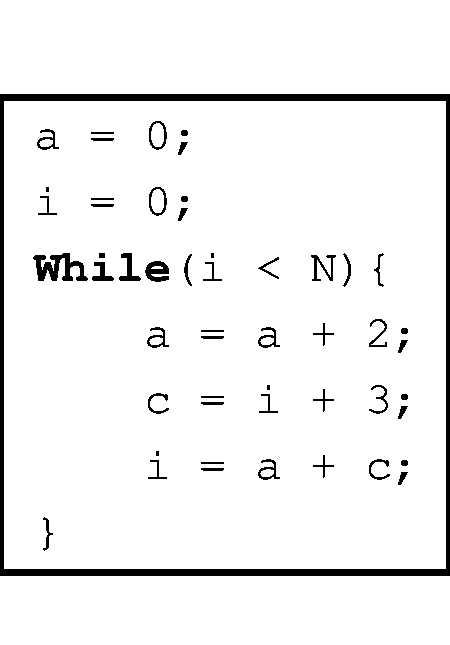
\includegraphics[height=1.8in]{fig-rpe/C-code}
& \hspace{2cm}
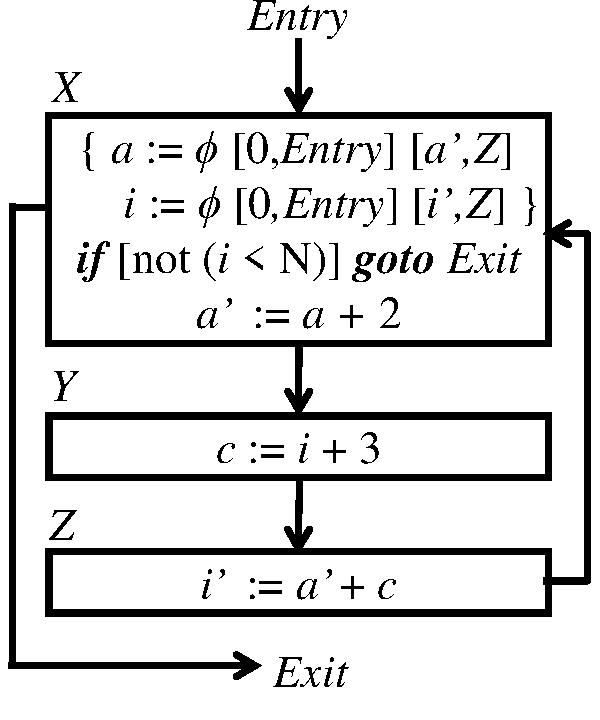
\includegraphics[height=1.8in]{fig-rpe/seq-ccdfg}
\\
(a) & \hspace{2cm} (b) 
\end{tabular}
\end{center}
\caption{(a) Loop in C (b) Loop CCDFG before pipelining.}
\label{fig:high-level-synthesis}
\end{figure}

Figure~\ref{fig:high-level-synthesis}(a) illustrates the C
code (ESL description) for a loop at the beginning of the
synthesis process. The C code does not have a schedule or the
concept of a clock cycle. Figure~\ref{fig:high-level-synthesis}(b)
shows CCDFG of the sequential loop just before loop pipelining. The loop has three scheduling steps: $X$, $Y$ and $Z$.  The scheduling step before the loop is $Entry$ and after the loop is $Exit$. Since,
there are three scheduling steps in the loop, one iteration
can be executed in three clock cycles.

\begin{figure}
\begin{center}
\begin{tabular}{cc}
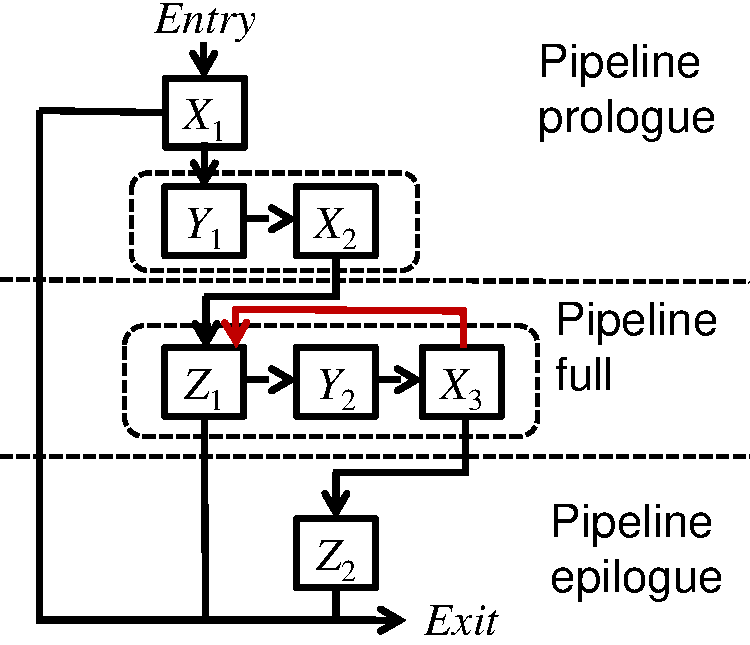
\includegraphics[height=1.8in]{fig-rpe/pipelined_ccdfg}
& \hspace{0.5cm}
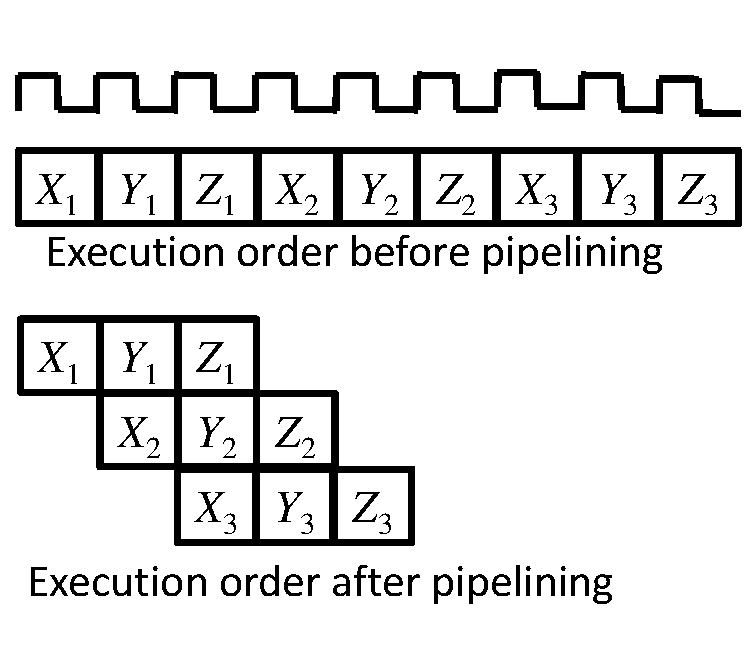
\includegraphics[height=1.8in]{fig-rpe/pp-clock-cycles}
\end{tabular}
\end{center}
\caption{Pipelined CCDFG. The horizontal arrows in the scheduling supersteps indicate data forwarding.}
\label{fig:pp-ccdfg}
\end{figure}

Behavioral synthesis tools use complicated heuristics and aggressive scheduling strategies to find an optimized pipeline interval (clock cycles after which a new iteration can be started such that there are no data hazards). Figure~\ref{fig:pp-ccdfg} shows the pipelined CCDFG with a pipeline interval equal to one. The new scheduling steps in the pipelined CCDFG created by combining scheduling steps from different iterations of the sequential CCDFG are called scheduling supersteps. Observe that the three iterations of the pipelined loop take five clock cycles as opposed to nine clock cycles in the sequential loop. Loop pipelining reduces the number of clock cycles required to execute the loop, hence this transformation is used by synthesis tools to increase throughput and reduce latency.  

\subsection{Correctness of Pipelined CCDFG}
\label{subsec:correctness-defn}

Loop Pipelining is a critical and complex transformation. So, it is important to certify that the pipelined CCDFG is indeed correct. Correctness of loop pipelining 
can be informally stated as below.

\begin{quote}
Let $L$ be a loop in CCDFG $C$, and let $L_{\alpha}$ be the
pipelined loop CCDFG. Let $V$ be the set of
variables mentioned in $L$, and $U$ be the set of all
variables in $C$.  Suppose we execute $L$ and $L_{\alpha}$
from CCDFG states $s$ and $s'$ respectively, such that for
each variable $v\in V$, the value of $v$ in $s$ is the same
as that in $s'$, and suppose that the state on termination
are $f$ and $f'$ respectively.  Then (1)~for any $v\in V$,
the value of $v$ in $f$ is the same as that in $f'$, and
(2)~for any $v\in(U\backslash V)$, the value of $v$ in $f'$
is the same as that in $s'$.
\end{quote}
\noindent
{\em Remark:} Condition (2) is the {\em frame rule} which
ensures that variables in $C$ that are not part of the loop
are not affected by $L_{\alpha}$.

\subsection{An approach to verification of loop pipelining transformation}
\label{subsec:hao-approach}

%Hao et al.~\cite{hrx:dac-12} develop a pipeline algorithm that takes as inputs these parameters and a CCDFG and generates a reference pipelined CCDFG. 
Hao {\em et al.} proposed a pipeline generation algorithm using feedback (like pipeline interval) from the synthesis tool~\cite{hrx:dac-12}. They show that to verify the correspondence between sequential CCDFG and pipelined RTL, it is sufficient to perform the following three steps. 
\begin{enumerate} 
\item Check that the algorithm can generate a pipeline reference model for the parameters reported by synthesis.
\item Use SEC to compare the pipeline reference model with the
synthesized RTL.
\item Prove the correctness of the algorithm. 
\end{enumerate}

The pipelining algorithm is simpler than that used by the synthesis tool because the synthesis tool uses advanced heuristics to determine the pipeline parameters 
(such as how many iterations to pipeline, when to introduce stalls etc.), while this pipelining algorithm only uses those parameters to generate a reference model. The algorithm is shown to be scalable but it is not certified. 

\medskip
\noindent {\bf The proposed algorithm}
\label{subsec:kecheng's algorithm}

\noindent
Given a set of microsteps $M$, a set of edges $E$, and a schedule $S$ of a
sequential CCDFG, and pipeline parameters (pipeline
interval $I$ and number of scheduling steps in the loop
$N$), the algorithm generates new microsteps, edges and
schedule for pipelined CCDFG by pipelining the
loops. Values of these inputs are readily available from
intermediate feedback reports from the behavioral synthesis
tool. Given CCDFG $C$, the reference transformation replaces
each loop $L$ in $C$ with the pipelined refinement of
$L$. The steps of the algorithm are explained below with the
help of the example introduced earlier
(cf. Figure~\ref{fig:high-level-synthesis}) .

%\medskip
%\begin{algorithm}
%\caption{Loop Pipelining Algorithm} \label{algo:hao}
%\begin{algorithmic}[1]
%\Procedure{PIPELINELOOP}{L=(S, E, M), I, N}
%\State $S_1 \leftarrow Generate Scheduling Steps (S, I, N)$.
%\State $(S_2, M_1) \leftarrow Generate Pipeline Regs (S_1, M, E, I)$.
%\State $ E_1 \leftarrow Generate Edges (S_2, E, I, N)$.
%\State $S_3, M_2) \leftarrow Generate Forwarding (S_2, M_1, E_1, I)$.
%\State \textbf{return} $(S_3, E_1, M_2)$.
%\EndProcedure
%\end{algorithmic}
%\end{algorithm}

\begin{figure}
\begin{center}
\begin{tabular}{cc}
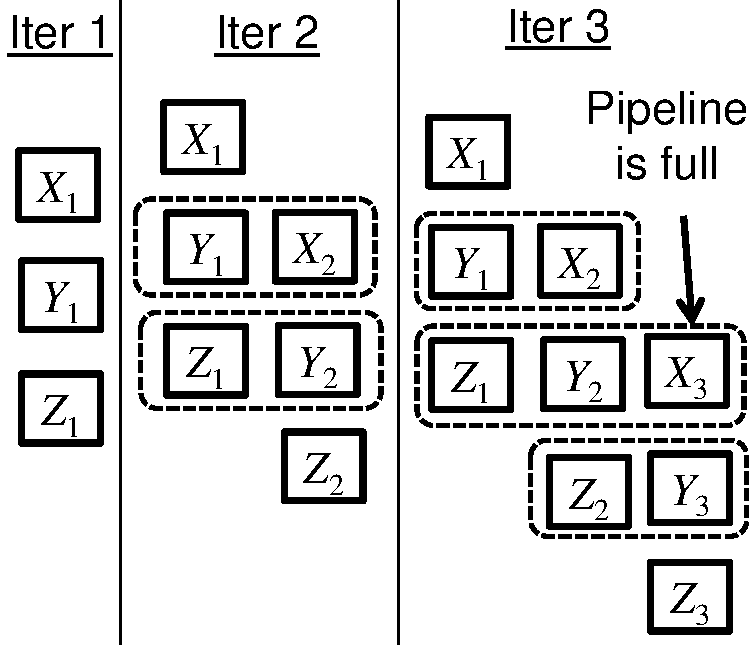
\includegraphics[height=1.7in]{fig-rpe/generate-scheduling-steps}
& %\hspace{0.1cm}
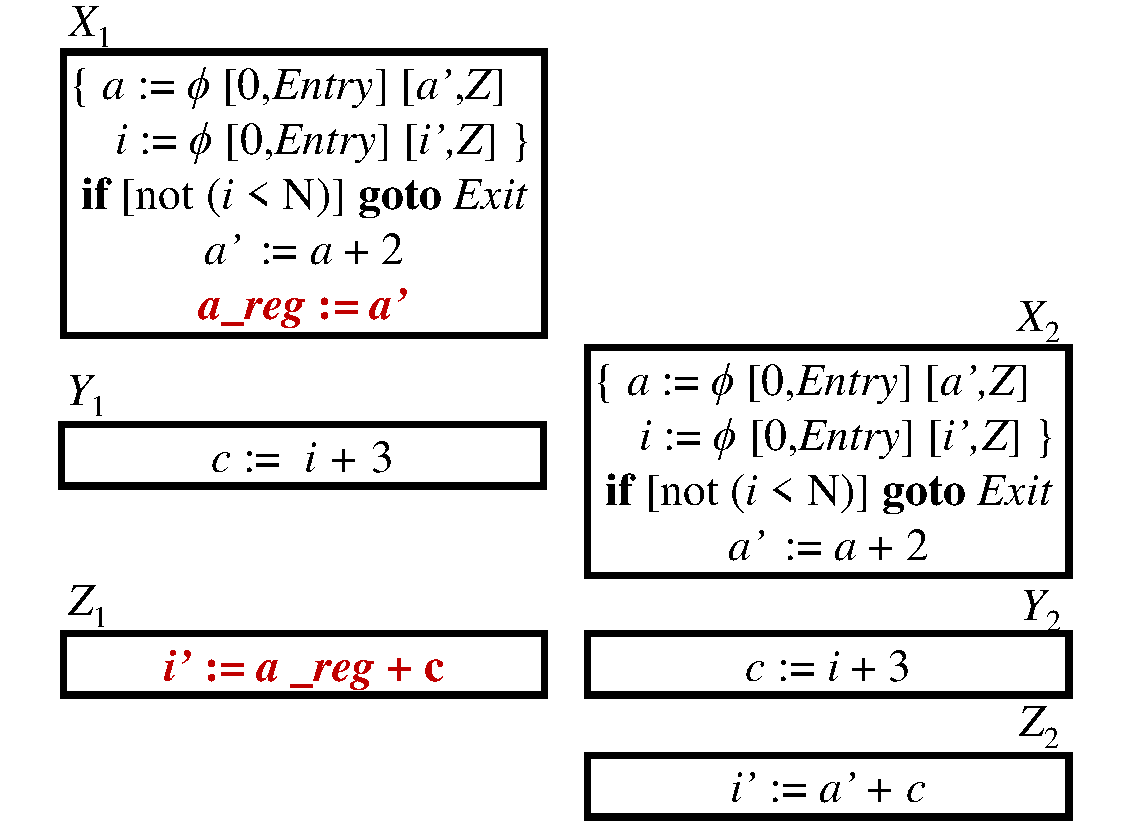
\includegraphics[height=1.7in]{fig-rpe/shadow-reg}
\\
(a) & (b)
\end{tabular}
\end{center}
\caption{(a) Generate scheduling steps. After the pipeline is full, adding new iteration simply repeats the pipeline full stage. (b) Generate shadow registers.}
\label{fig:algorithm}
\end{figure}

\begin{enumerate}
\item {\bf Generate scheduling steps:} Figure~\ref{fig:algorithm}(a) shows the addition of scheduling steps of new iterations of a loop according to the pipeline interval. Here, the loop has three scheduling steps and a pipeline interval of one. The new scheduling steps are generated till the pipeline is full. This step generates a new schedule. 

\item {\bf Generate shadow registers:} In order to pipeline a loop, we have to get rid of data hazards. We first identify all variables that can be overwritten and then introduce new variables called shadow registers. In Figure~\ref{fig:algorithm}(b), the value of $a'$ will be overwritten in $X_2$ before $Z_1$ can read it. So, we introduce a new pipeline register $a\_reg$ which gets assigned the value of $a'$ and replace subsequent reads of $a'$ with reads of $a\_reg$.

\begin{figure}[t!]
\begin{center}
\begin{tabular}{cc}
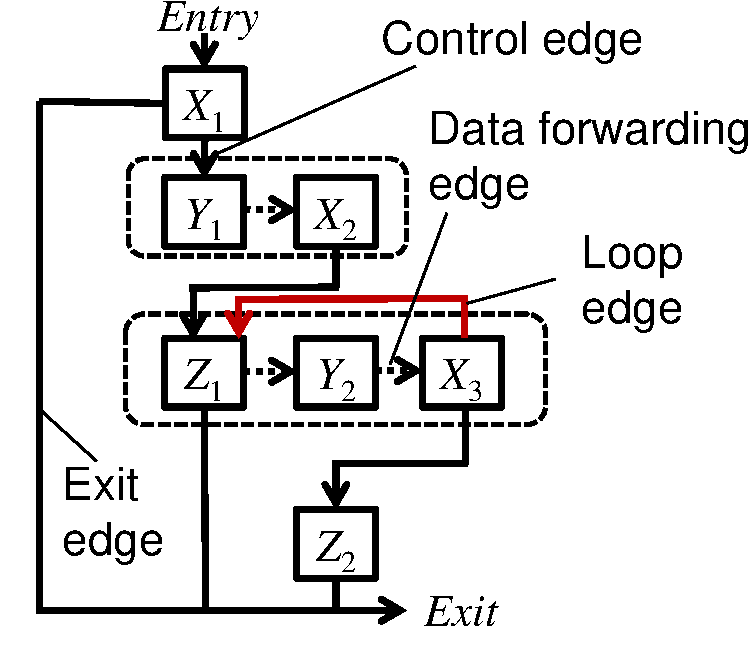
\includegraphics[height=1.7in]{fig-rpe/generate-edges}
& %\hspace{0.1cm}
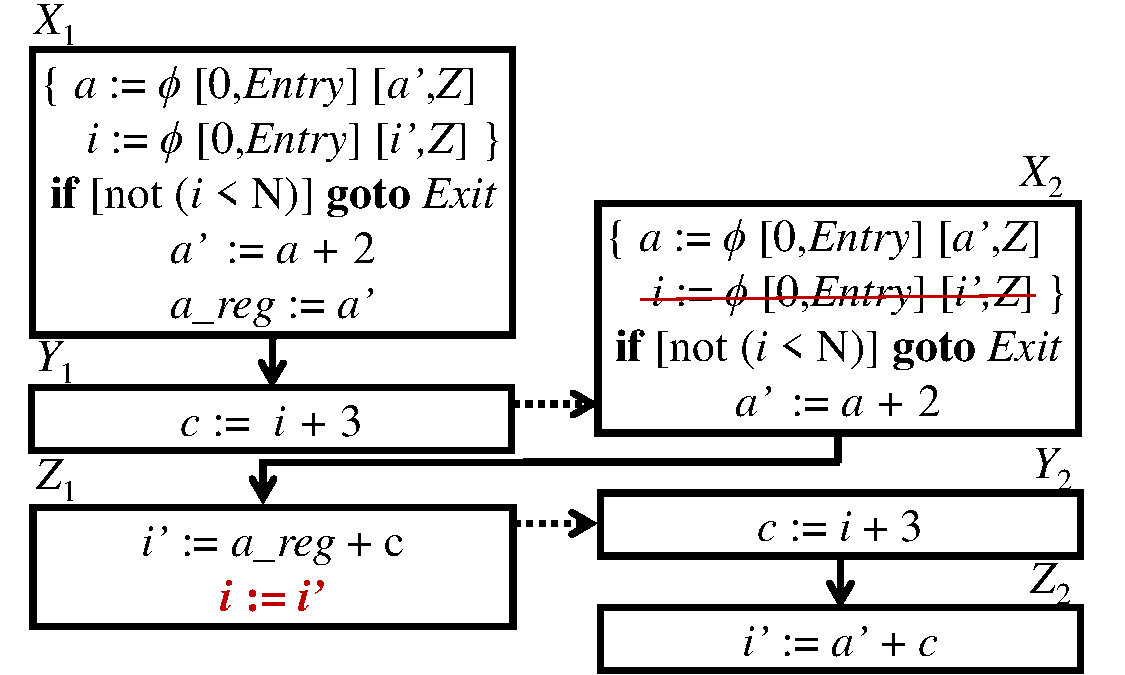
\includegraphics[height=1.7in]{fig-rpe/data-forwarding}
\\
(a) & (b)
\end{tabular}
\end{center}
\caption{(a) Generate Edges for pipelined CCDFG (b) Data propagation.}
\label{fig:algorithm-2}
\end{figure}
 
\item {\bf Generate edges:} The algorithm adds the edges for data and control flow as shown in Figure~\ref{fig:algorithm-2}(a). Control edges are edges from one scheduling superstep to the next. Data forwarding edges forward data from one scheduling step to the next in a single scheduling superstep. Loop edge denotes the repetition of the full pipeline stage. Exit edges are from the scheduling steps to the $Exit$ block. Note, a pipelinable loop has only one $Exit$ block.

\item {\bf Generate data propagation:} In Figure~\ref{fig:algorithm-2}(b), we require the value of $i'$ in $X_2$ to execute the following statement:
$$ i := \phi [0, Entry][i', Z]$$
But, if we execute $X_2$ before executing $Z_1$, the value of $i'$ has not yet been produced. To avoid such a situation, we relocate the assignment statement $i := i'$ to $Z_1$. Note, the assignment statement $i := i'$ is obtained from the $\phi$-statement $i := \phi [0, Entry][i', Z]$ since in sequential execution, we would have entered $X_2$ from $Z$ block.
\end{enumerate}
